\section{Library of transformations}

\begin{frame}{The library}
    The library of transformations contains small transformation steps that are proven correct.
    \begin{itemize}
        \item Each transformation in here can be used as building block.
        \item The library of transformations does not achieve complete coverage.
    \end{itemize}
\end{frame}

\note{
	\begin{itemize}
	    \item Explain what the library of transformations is.
	    \item Explain that the library included within this work is incomplete, e.g. not all possible models can be build from this library.
	    \item Explain in context what the library of transformations is.
	\end{itemize}
}

\begin{frame}{In context}
    \begin{columns}[c]
        \begin{column}{0.05\textwidth}
        \end{column}\begin{column}{0.3\textwidth}
            \centering
            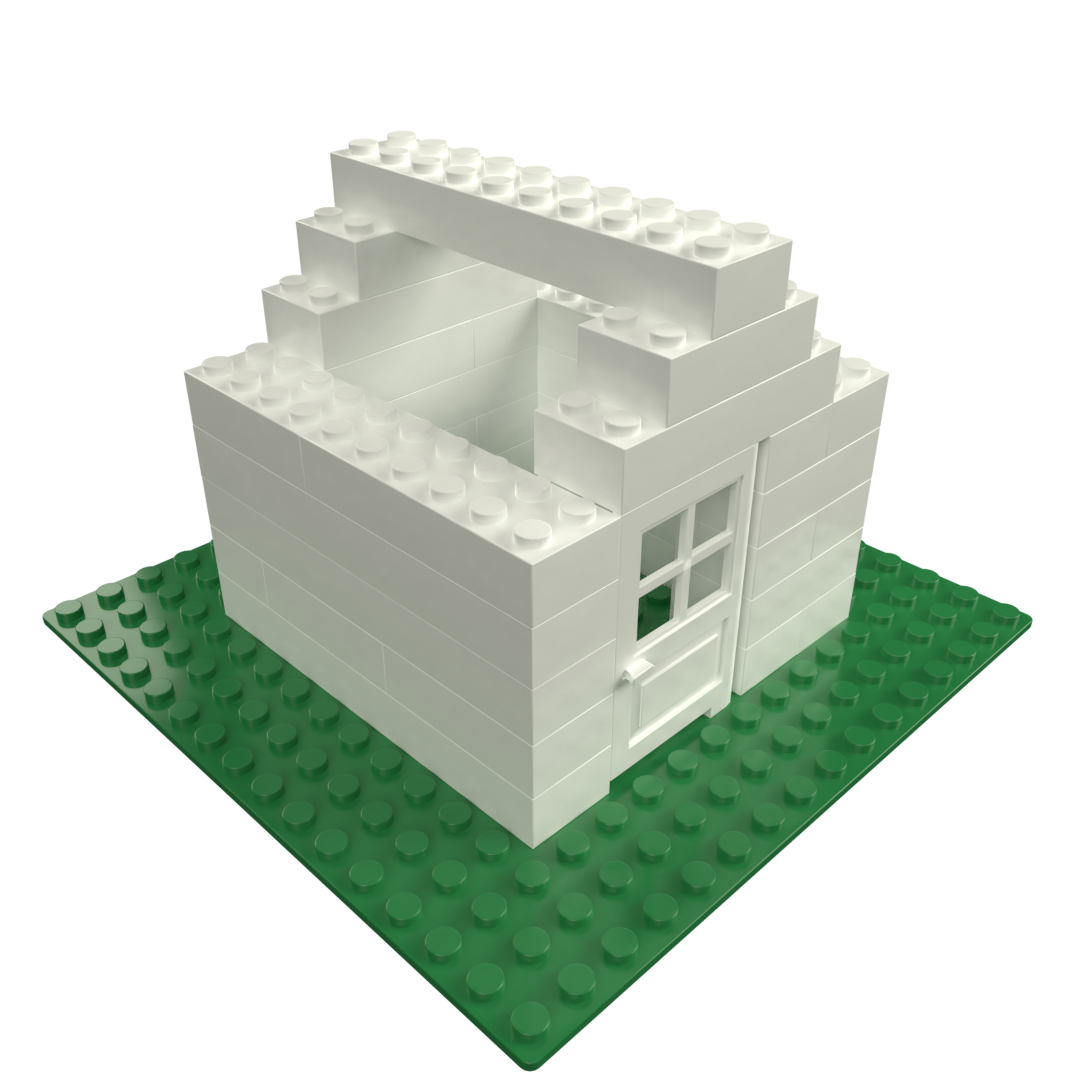
\includegraphics[width=0.7\textwidth]{images/03_transformation_framework/lego_house_roofless.png}
        \end{column}\begin{column}{0.05\textwidth}
            \centering
            +
        \end{column}\begin{column}{0.2\textwidth}
            \centering
            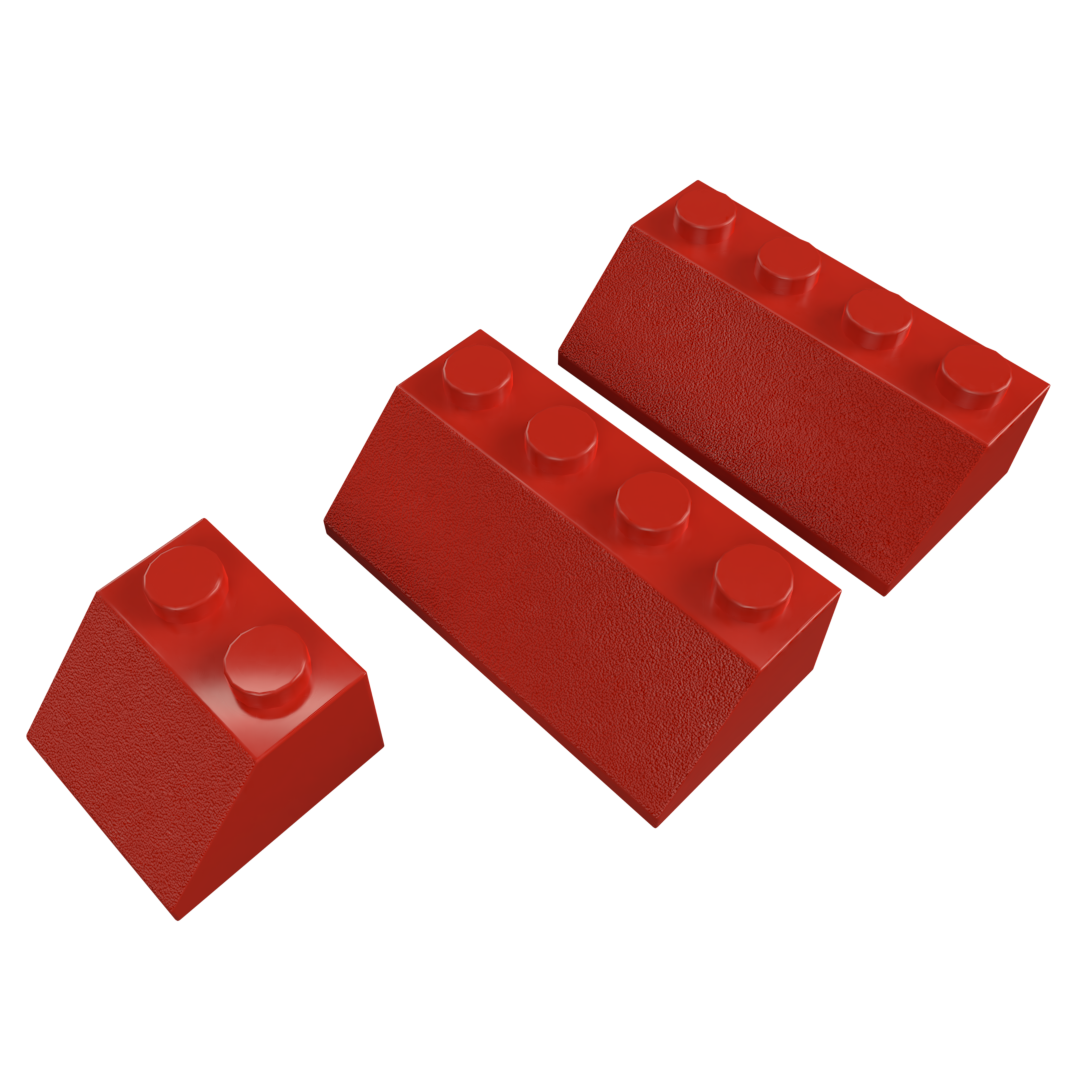
\includegraphics[width=0.7\textwidth]{images/03_transformation_framework/lego_roof_pieces.png}
        \end{column}\begin{column}{0.05\textwidth}
            \centering
            =
        \end{column}\begin{column}{0.3\textwidth}
            \centering
            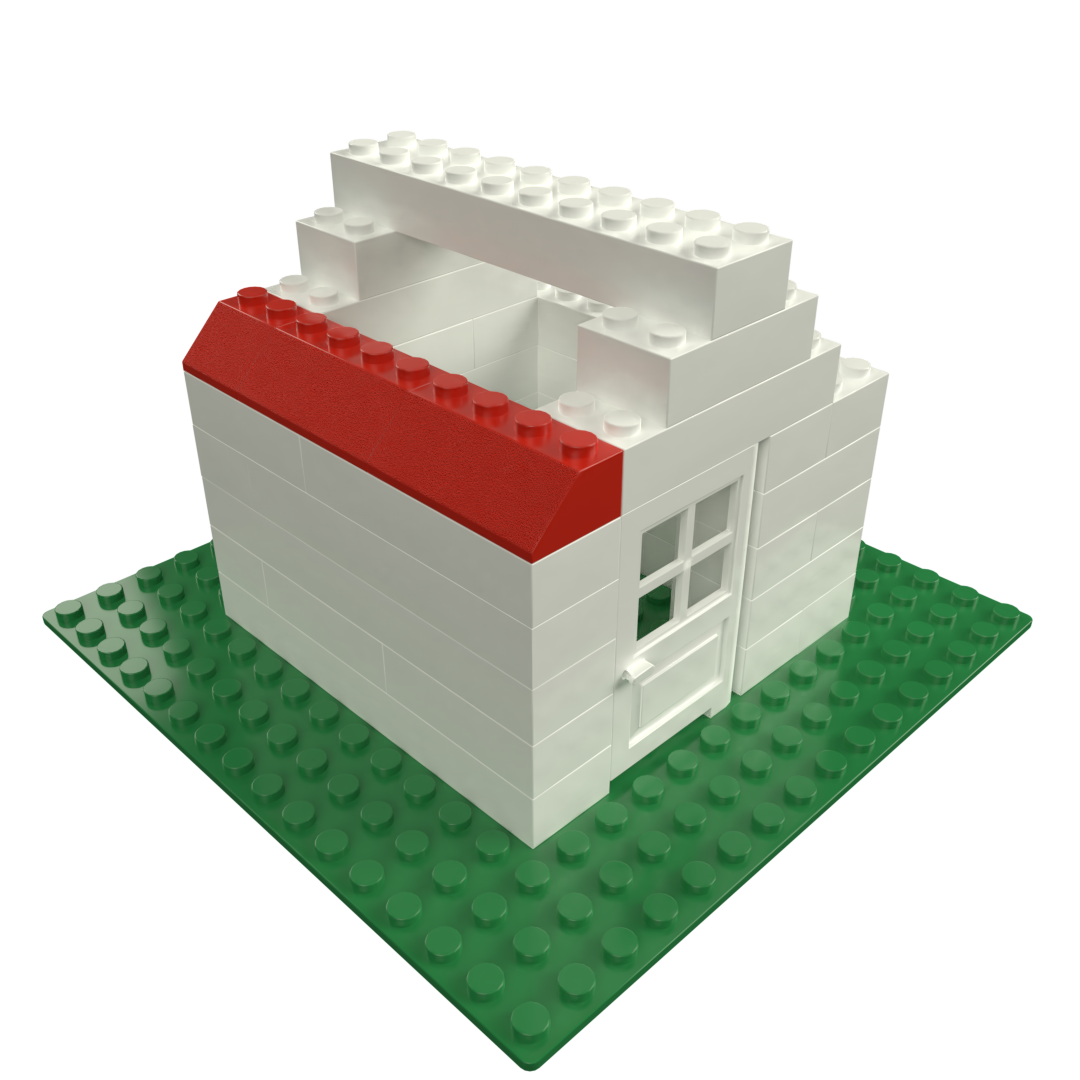
\includegraphics[width=0.7\textwidth]{images/03_transformation_framework/lego_house_roof_step.png}
        \end{column}
    \end{columns}
    \begin{columns}[c]
        \begin{column}{0.05\textwidth}
        \end{column}\begin{column}{0.3\textwidth}
            \centering
            \rotatebox{90}{$\leftrightarrow$}
        \end{column}\begin{column}{0.05\textwidth}
            \centering
            $\sqcup$
        \end{column}\begin{column}{0.2\textwidth}
            \centering
            \rotatebox{90}{$\leftrightarrow$}
        \end{column}\begin{column}{0.05\textwidth}
            \centering
            =
        \end{column}\begin{column}{0.3\textwidth}
            \centering
            \rotatebox{90}{$\leftrightarrow$}
        \end{column}
    \end{columns} 
    \begin{columns}[c]
        \begin{column}{0.05\textwidth}
        \end{column}\begin{column}{0.3\textwidth}
            \centering
            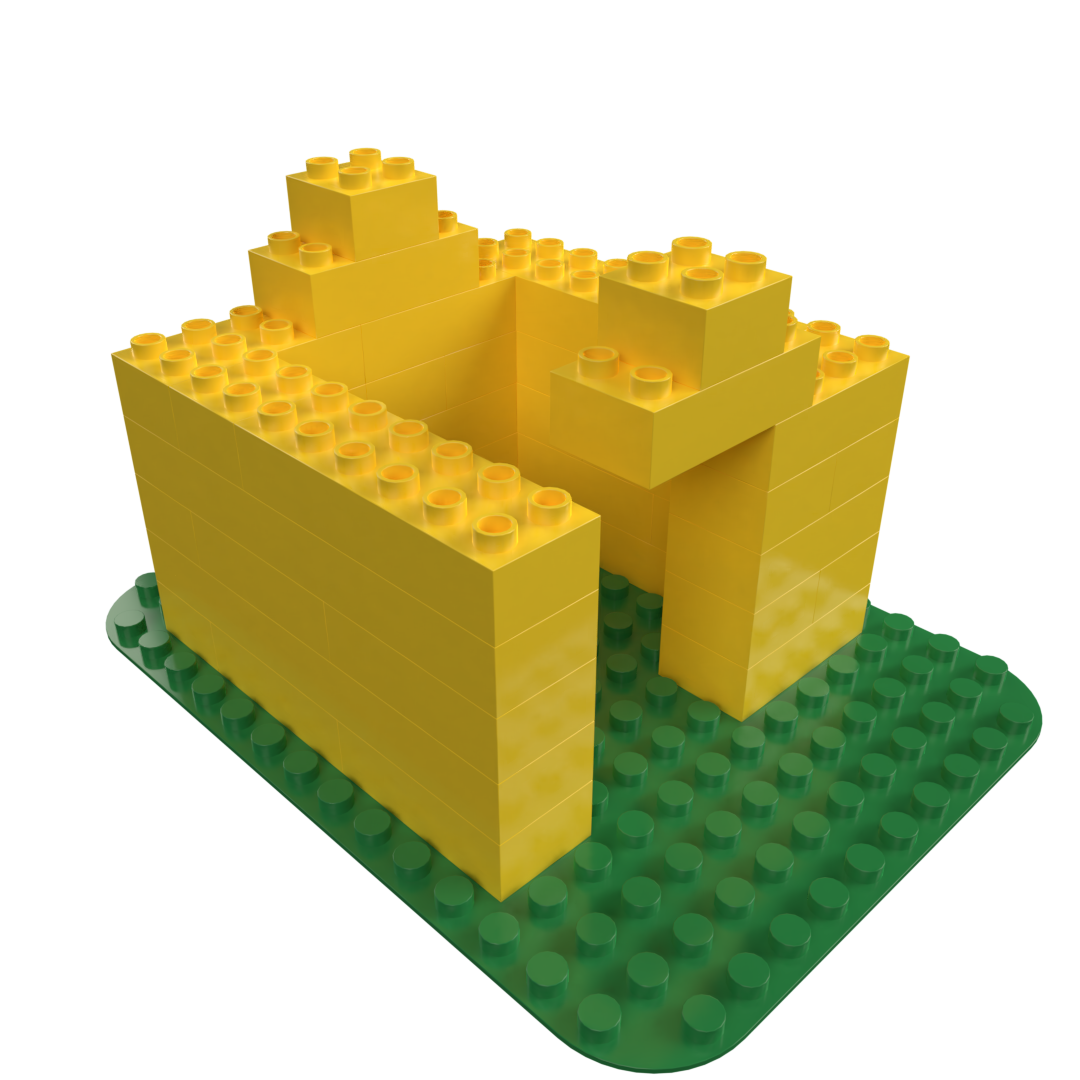
\includegraphics[width=0.7\textwidth]{images/03_transformation_framework/duplo_house_roofless.png}
        \end{column}\begin{column}{0.05\textwidth}
            \centering
            +
        \end{column}\begin{column}{0.2\textwidth}
            \centering
            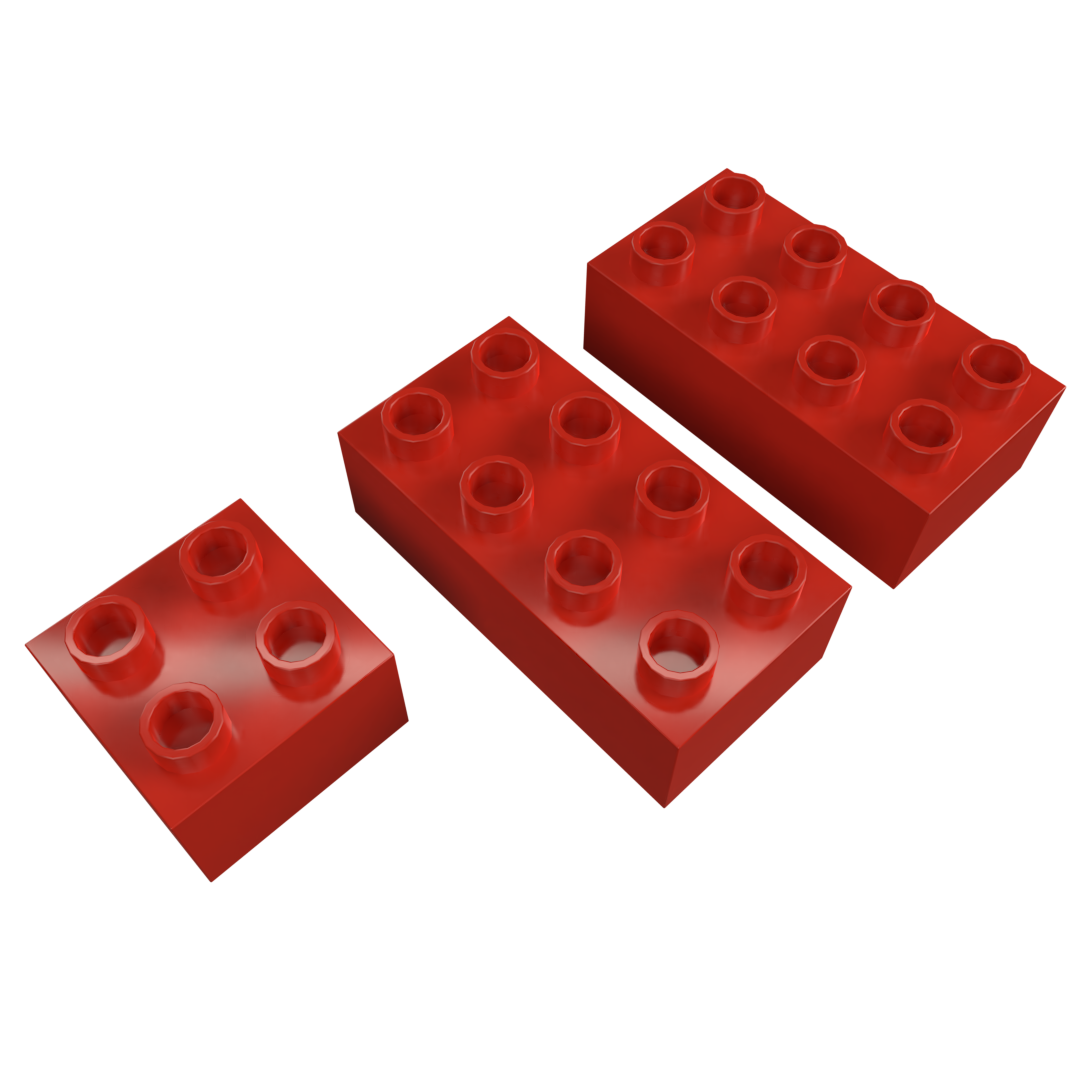
\includegraphics[width=0.7\textwidth]{images/03_transformation_framework/duplo_roof_pieces.png}
        \end{column}\begin{column}{0.05\textwidth}
            \centering
            =
        \end{column}\begin{column}{0.3\textwidth}
            \centering
            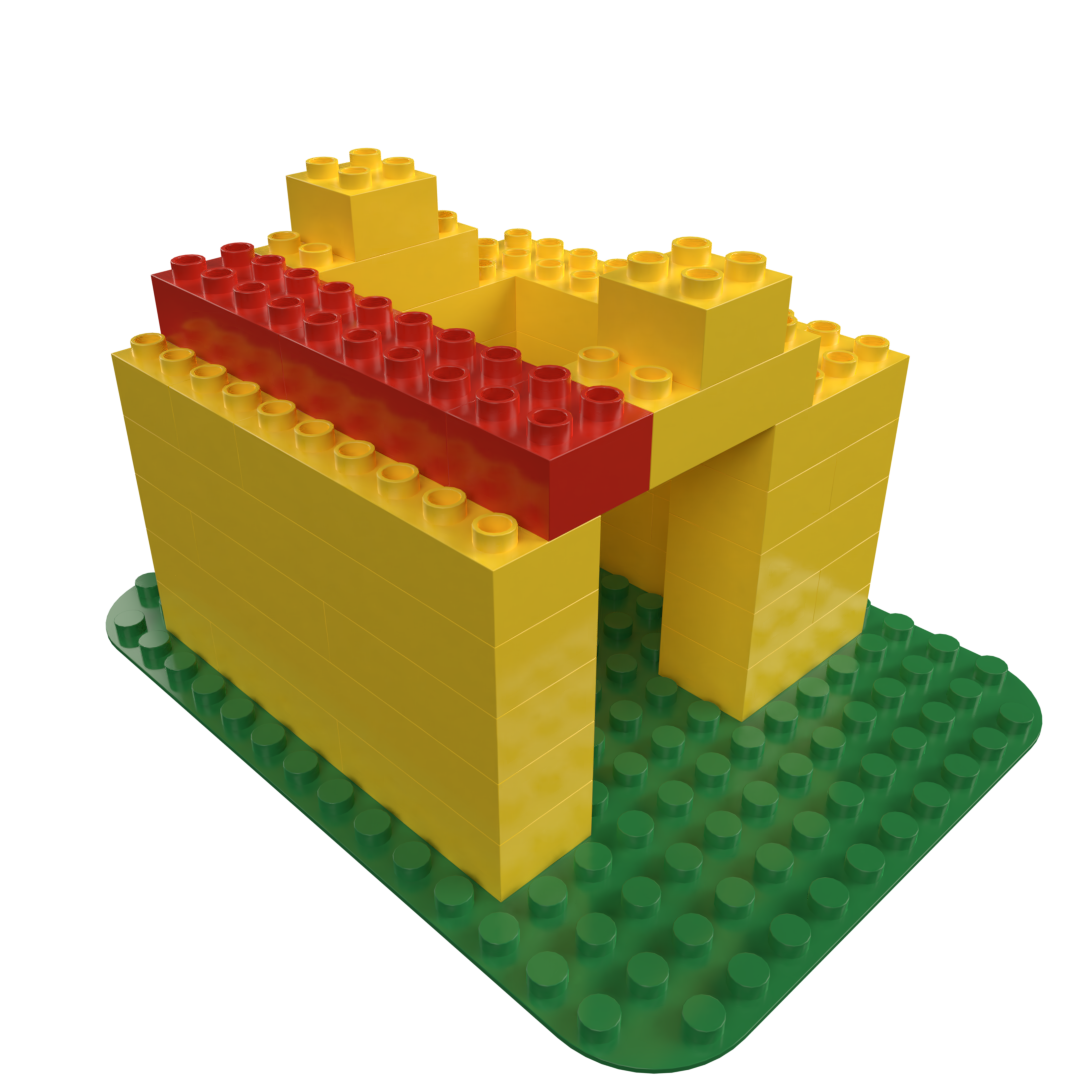
\includegraphics[width=0.7\textwidth]{images/03_transformation_framework/duplo_house_roof_step.png}
        \end{column}
    \end{columns} 
\end{frame}

\begin{frame}{Adding a regular class with instances}
Add a class named \textit{Example} to a model. On the instance level, introduce a set of objects with this type.
\begin{columns}[c]
    \begin{column}{0.05\textwidth}
    \end{column}\begin{column}{0.45\textwidth}
        \centering
        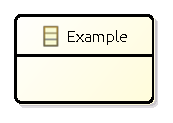
\includegraphics[width=0.5\textwidth]{images/04_library_of_transformations/class_type.pdf}
    \end{column}\begin{column}{0.05\textwidth}
        \centering
        $\leftrightarrow$
    \end{column}\begin{column}{0.45\textwidth}
        \centering
        % To use this figure in your LaTeX document
% import the package groove/resources/groove2tikz.sty
%
\begin{tikzpicture}[scale=\tikzscale,name prefix=test-]
\node[type_node] (n0) at (0.950, -0.850) {\ml{\textbf{Example}}};

\end{tikzpicture}

    \end{column}
\end{columns}
\begin{columns}[c]
    \begin{column}{0.05\textwidth}
    \end{column}\begin{column}{0.45\textwidth}
        \centering
        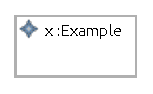
\includegraphics[width=0.5\textwidth]{images/04_library_of_transformations/class_instance.pdf}
    \end{column}\begin{column}{0.05\textwidth}
        \centering
        $\leftrightarrow$
    \end{column}\begin{column}{0.45\textwidth}
        \centering
        % To use this figure in your LaTeX document
% import the package groove/resources/groove2tikz.sty
%
\begin{tikzpicture}[scale=\tikzscale,name prefix=start-]
\node[basic_node] (n0) at (1.620, -0.370) {\ml{\uline{\textit{x}} : \textbf{Example}}};

\end{tikzpicture}

    \end{column}
\end{columns}
\end{frame}

\note{
	\begin{itemize}
	    \item Shortly explain what a transformation within the library looks like. It has a type level transformation with corresponding instance level transformations.
	    \item Very quickly explain the model and how to apply it.
	\end{itemize}
}

\begin{frame}{Adding a string field}
Add a field, typed by a string, named \textit{field} to an existing class named \textit{Example}. For all existing objects typed by \textit{Example}, introduce a new value for the field \textit{field}.
\begin{columns}[c]
    \begin{column}{0.05\textwidth}
    \end{column}\begin{column}{0.45\textwidth}
        \centering
        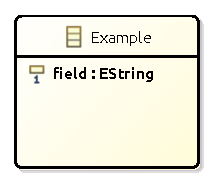
\includegraphics[width=0.7\textwidth]{images/04_library_of_transformations/data_field.pdf}
    \end{column}\begin{column}{0.05\textwidth}
        \centering
        $\leftrightarrow$
    \end{column}\begin{column}{0.45\textwidth}
        \centering
        % To use this figure in your LaTeX document
% import the package groove/resources/groove2tikz.sty
%
\begin{tikzpicture}[scale=\tikzscale,name prefix=test-]
\node[type_node] (n0) at (0.955, -0.775) {\ml{\textbf{Example}\\field: \textbf{string}}};

\end{tikzpicture}

    \end{column}
\end{columns}
\begin{columns}[c]
    \begin{column}{0.05\textwidth}
    \end{column}\begin{column}{0.45\textwidth}
        \centering
        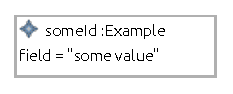
\includegraphics[width=0.7\textwidth]{images/04_library_of_transformations/data_field_value.pdf}
    \end{column}\begin{column}{0.05\textwidth}
        \centering
        $\leftrightarrow$
    \end{column}\begin{column}{0.45\textwidth}
        \centering
        % To use this figure in your LaTeX document
% import the package groove/resources/groove2tikz.sty
%
\begin{tikzpicture}[scale=\tikzscale,name prefix=start-]
\node[basic_node] (n0) at (1.595, -0.775) {\ml{\uline{\textit{someId}} : \textbf{Example}\\field = "some value"}};

\end{tikzpicture}

    \end{column}
\end{columns}
\end{frame}

\note{
	\begin{itemize}
	    \item Explain the addition of a string field as last example.
	\end{itemize}
}